\chapter{Les phonons}
Ce chapitre traîte des ions dans un corps cristallin : fournir de l'énergie à 
un ion du réseau va entraîner une redistribution rapide de celle-ci dans le 
cristal par interactions entre ions : un phénomène local conduit à des vibrations 
collectives de tout le système. On introduit alors des coordonnées collectives. En 
effet, les vibrations peuvent être quantifiées et un quanta de cette excitation 
n'est rien d'autre qu'un phonon, qui est aussi boson et donc décrit par 
Bose-Einstein.

\section{L'énergie d'un réseau 1D dans l'approximation harmonique}
Analysons les vibrations d'une chaîne linéaire d'atomes identiques de masse 
$M$ séparé de $a$ (constante de réseau) à l'équilibre. Soit $y_R$ le déplacement 
de l'atome $R$ à partir de sa position d'équilibre $R$ de sorte que sa position 
soit $R+y_R$. On peut écrire l'hamiltonien d'un tel système 
\begin{equation}
\mathcal{H} = \sum_R \dfrac{p_R^2}{2M}+\mathcal{V}(\dots,y_R,\dots,y_{R'},\dots)
\end{equation}
On peut développer le potentiel en série de Taylor
\begin{equation}
\mathcal{V}(\dots,y_R,\dots,y_{R'},\dots) = V_0(0,0,\dots) + \sum_R y_R\left(
\dfrac{\partial \mathcal{V}}{\partial y_R}\right)_0 + \frac{1}{2!}\sum_{R\ R'} 
y_Ry_{R'}\left(\dfrac{\partial^2\mathcal{V}}{\partial y_R\partial y_{R'}}\right)_0 
+\dots
\end{equation}
L'approximation harmonique revient à supprimer les termes plus grand que le 
terme quadratique. Le premier terme, lui, peut être nul en faisant un bon choix 
pour l'origine des énergie tandis que le second terme également : les dérivées 
premières doivent être nulles car à l'équilibre un atome n'est soumise à aucune 
force. On considère donc
\begin{equation}
\mathcal{V}_2 =  \frac{1}{2!}\sum_{R\ R'} 
y_Ry_{R'}\left(\dfrac{\partial^2\mathcal{V}}{\partial y_R\partial y_{R'}}\right)_0 =
\dfrac{1}{2}\sum_{R\ R'} y_RV_{RR'}y_{R'}
\end{equation} 
Comme $V_{RR'}$ est hermitique ($V_{RR'} = V_{R'R}^*$), elle est peut être (ce 
qui n'est pas encore le cas) diagonalisée par une transformation unitaire. Comme 
les atomes sont identiques et indiscernables, $y_R$ ne dépend que de $R$ (du 
réseau de Bravais). Dès lors, la matrice $U_{qR} = e^{iqR}$ réalise cette 
transformation. Considérons le développement de Fourier suivant
\begin{equation}
y_R = \dfrac{1}{\sqrt{N}}\sum_q y_qe^{iqR}
\label{eq:DevFourier}
\end{equation}
où $N$ est le nombre de mailles du réseau. On peut introduire le conjugué hermitique 
de cette observable
\begin{equation}
y_{R'} = y_{R'}^+ = \dfrac{1}{\sqrt{2}}\sum_{q'} y_{q'}^+ e^{-iq'R'}
\end{equation}
On peut ré-écrire $\mathcal{V}_2$ (Le + vient du fait qu'il soit hermitique, et 
on substitue les termes) : 
\begin{equation}
\begin{array}{ll}
\mathcal{V}_2 & \displaystyle \frac{1}{2}\sum_{R\ R'} y_R V_{RR'}y_{R'}^+ = 
\frac{1}{2N}\sum_{RR'}{qq'} V_{RR'} y_qe^{iqR}e^{-iq'R'}\\
 & \displaystyle \dfrac{1}{2N}\sum_{R\ R'}\sum_{q\ q'} V_{R-R'}e^{eq(R-R')}y_q
 e^{i(q-q')R'}y_{q'}^+
\end{array}
\end{equation}
Le potentiel $V_{RR'}$ est en fait un potentiel $V_{R-R'}$ qui ne dépend que de la 
périodicité du réseau de Bravais. Posons $L = R-R'$, la distance entre les ions 
$R$ et $R'$. La somme sur $R$ peut être remplacée par la somme sur $L$ (mais on 
garde la somme sur $R'$)\footnote{On peut ? Comment?} :
\begin{equation}
\mathcal{V}_2 = \dfrac{1}{2N}\sum_{qq'}\left(\sum_L V_L e^{iqL}\right)y_q\left(
\sum_{R'} e^{i(q-q')R'}\right)y_q^+
\end{equation}
Posons $\displaystyle V_q = \sum_L e^{iqL}V_L$. On obtient finalement
\begin{equation}
\mathcal{V}_2 = \frac{1}{2}\sum_q V_qy_qy_q^+
\end{equation}
Il est possible de déterminer 
la valeur de la somme sur $R'$ grâce aux CL. Comme on ne peut pas dépasser le 
nombre de mode indépendants, on va considérer que le cristal se refermait sur 
lui-même : il s'agit des CL de Born-Von-Kerman qui vont introduire la 
quantification du vecteur $q$.\\
La valeur de la somme étant indépendante de l'atome de départ :
\begin{equation}
\mathcal{S} = \sum_R e^{i(q-q')R} = \sum_{l=1}^N e^{i(q-q')la} = \sum_{l=2}^{N+1} 
e^{i(q-q')la} = \sum_{l=1}^N e^{i(q-q')(l+1)a} = e^{i(q-q')a}\mathcal{S}
\end{equation}
La somme $\mathcal{S}$ est donc nulle, sauf si $q=q'$ et dans ce cas, elle vaut 
$N$. On trouve donc 
\begin{equation}
\sum_R e^{i(q-q').R} = N\delta_{qq'}
\end{equation}
Nous avons ici fait des sommes sur des exponentielles complexes. Physiquement, 
nous avons donc sommé des phases donnant lieu à des interférences. Ces 
interférences seront 
\begin{multicols}{2}
\begin{itemize}
\item[$\bullet$] Constructives si $q=q'$
\item[$\bullet$] Destructrices si $q\neq q'$
\end{itemize}
\end{multicols}
Nous avons donc diagonalisé le terme quadratique $\mathcal{V}_2$. En effet, on 
peut l'écrire avec une somme de termes dépendant chacun d'une \textit{coordonnée 
collective} $y_q$ qui représente l'amplitude d'une onde impliquant les déplacement 
$y_R$ de tous les ions du cristal. On peut en effet considérer le "développement 
de Fourier inverse" :
\begin{equation}
y_q = \frac{1}{\sqrt{N}}\sum_R y_Re^{-iqR}
\end{equation}
On peut vérifier la validité de cette expression en la substituant dans 
\autoref{eq:DevFourier}.\\
La coordonnée collective $p_q$, canoniquement conjuguée à $y_q$ à la forme
\begin{equation}
p_q = -i\hbar \dfrac{\partial}{\partial y_q} = \sum_R \left(-i\hbar\dfrac{
\partial}{\partial y_R}\right)\dfrac{\partial y_R}{\partial y_q} = \dfrac{1}{
\sqrt{2}}\sum_R p_R e^{iqR}
\end{equation}
On peut vérifier que la transformation inverse\footnote{C'est-à-dire?} est
\begin{equation}
p_R = \frac{1}{\sqrt{N}} \sum_q p_q e^{-iqR}
\end{equation}
Comme $p_R$ est une observable, nous avons
\begin{equation}
p_R = p_R^+ = \frac{1}{\sqrt{N}}\sum_{q'} p_{q'}^+ e^{iq'R}
\end{equation}
Compte-tenu de ces nouvelles relation, on peut écrire l'énergie cinétique 
à l'aide des impulsions collectives $p_q$ : 
\begin{equation}
\frac{1}{2M}\sum_R p_R^2 = \dots = \frac{1}{2M}\sum_q p_qp_q^*
\end{equation}
En posant $M\omega_q^2 = V_q$ pour faire apparaître la pulsation (et pour 
plus tard faire apparaître les modes quantifiés et le relation de dispersion), 
notre hamiltonien devient
\begin{equation}
\mathcal{H} = \sum_q \left[\frac{1}{2M}p_qp_q^+ + \dfrac{1}{2}M\omega_q^2 y_q
y_q^+\right]
\end{equation}
ce qui n'est rien d'autre qu'une somme d'hamiltonien d'oscillateurs harmoniques.\\
Avec la définition de $p_q$, les relations de commutation sont les mêmes pour 
les coordonnées collectives que pour les particules
\begin{equation}
[y_q,p_{q'}] = i\hbar\delta_{qq'},\qquad [y_q^+,p_{q'}^+] = i\hbar\delta_{qq'}
\end{equation}
Définissons les opérateurs abaisseurs (diminue de une unité le nombre de 
phonons) et remonteurs (l'inverse)(cf. \textit{Mécanique Quantique I}) :
\begin{equation}
\begin{array}{ll}
a_q &= \displaystyle \sqrt{\dfrac{1}{2M\hbar\omega_q}}(M\omega_qy_q+ip_q^+)\\
a_q^+ &= \displaystyle \sqrt{\dfrac{1}{2M\hbar\omega_q}}(M\omega_qy_q-ip_q^+)
\end{array}
\end{equation}
On obtient alors
\begin{equation}
\mathcal{H} = \sum_q \hbar \omega_q (a^+a+\frac{1}{2})
\end{equation}
Par facilité, on considère des CL périodiques :
\begin{equation}
y_{R+Na} = y_R
\end{equation}
où $a$ est la distance entre atomes (la chaîne d'atomes est ainsi "jointe"). 
D'après \autoref{eq:DevFourier}, si les valeurs de $y_q$ sont uniques, on a 
\begin{equation}
e^{iqR} = e^{iq(R+Na)}
\end{equation} 
Las valeurs possibles de $q$ sont 
\begin{equation}
q = \dfrac{2\pi n}{Na}\qquad n \in \mathbb{Z}
\end{equation}
Il en résulte que 
\begin{equation}
y_q \equiv y_{q+K},\qquad\qquad p_q \equiv p_{q+K}
\end{equation}
où $K$ est un multiple de $2\pi/a$. Les pulsations $\omega_q$ (ou l'énergie 
$\hbar\omega_q$) des phonons du mode de vibration $q$ sont donné par 
\begin{equation}
\omega_q = \sqrt{\dfrac{V_q}{M}}
\end{equation}
Vu ce que l'on vient de voir, $\omega_q$ à la périodicité du réseau 
réciproque :
\begin{equation}
\omega_q = \omega_{q+K}
\end{equation}
Il s'agit maintenant de trouver la relation de dispersion (la fréquence 
ou l'énergie en fonction du nombre d'onde $q$). Pour se faire, nous allons 
écrire l'équation du mouvement comme si les atomes étaient accrochés par 
des ressorts. \\
L'équation du mouvement de l'atome $R$ s'écrit
\begin{equation}
M \dfrac{d^2y_R}{dt^2} = K[(y_{R+a}-y_R)-(y_R-y_{R-a})] = K[y_{R+a}+y_{R-a}
-2y_R] = -\dfrac{\partial \mathcal{V}_2}{\partial y_k}
\end{equation}
de sorte que\footnote{??}
\begin{equation}
\begin{array}{lll}
\dfrac{\partial^2\mathcal{V}_2}{\partial y_R\partial y_{R'}} = V_{RR'} &= 2K
& \text{ si } R = R'\\
&= -K & \text{ si } R = R\pm a\\
&= 0 & \text{ autrement }
\end{array}
\end{equation}
On a alors
\begin{equation}
V_q = 2K-K(e^{iqa}+e^{-iqa}) = 4K\sin^2\dfrac{qa}{2}
\end{equation}
et 
\begin{equation}
\omega_q = 2\sqrt{\dfrac{K}{M}}|\sin\dfrac{qa}{2}|
\end{equation}
La fréquence maximale vaut $\omega_m = 2\sqrt{K/M}$ aux limites $q=\pm\pi/a$ 
de la première zone de Brillouin. Pour de grandes longueur d'onde, on retrouve 
un comportement de ligne continue. La vitesse de propagation est indépendante 
de la fréquence\footnote{$\sin x \approx x$ pour $x\rightarrow 0$.}
\begin{equation}
\omega_q \approx \sqrt{\dfrac{K}{M}}qa = v_0q,\qquad v_0 = \sqrt{\dfrac{Ka^2
}{M}}
\end{equation}
Notons que le fait que la ligne soit composée d'atome modifie la propagation 
lorsque $q$ est proche de la limite de la zone.


\section{Réseau à trois dimensions}
La difficulté n'est pas beaucoup plus grande, il faudra juste considérer 
plus d'indices et donc plus de lourdeur dans l'écriture. Commençons par un 
réseau de Bravais pour lequel $\vec{R}$ entre deux atomes peut toujours 
s'écrire
\begin{equation}
\vec{R} = l_1\vec{a_1}+l_2\vec{a_2}+l_3\vec{a_3}
\end{equation}
Notre potentiel va toujours dépendre de la dérivation des atomes et sera 
donc fonction des $y_R$. Par analogie, on peut écrire\footnote{Tous les 
$R$ sont en réalité vectoriels.}
\begin{equation}
\mathcal{H} = \sum_{R\ i} \frac{1}{2M}(p_R^l)^2 + \frac{1}{2}\sum_{RR, ij}
y_R^iy_R^jV_{RR'}^{ij} + \dfrac{1}{3!}\sum_{RR'R",ijk} y_K^iy_K^j y_K^k 
V_{RR'R"}^{ijk} + \dots
\end{equation}
Les quantités tensorielles ($V_{RR'}^{ij},\dots$) sont les dérivées de 
l'énergie potentielle par rapport aux déplacements, comme avant. Seuls les 
deux premiers termes sont retenus dans l'approximation harmonique, 
permettant l'écriture de $\mathcal{H}$ sous forme matricielle.\\
Comme en $1D$, on peut définir des variables collectives\footnote{De même, 
les $q$ sont des vecteurs.} :
\begin{equation}
y_q^i= \dfrac{1}{\sqrt{N}}\sum_R y_R^i e^{-iq.R},\qquad p_q^i = \frac{1}{
\sqrt{N}}\sum_R p_K^i e^{iq.R}
\end{equation}
Il en résulte que $y_{q+K} \equiv y_q$ et $p_{q+K} \equiv p_q$ pour chaque 
$\vec{K}$ du réseau réciproque. Généralement, on restreint $q$ à la première 
zone de Brillouin. Cette restriction permet l'écriture des transformations 
inverses comme précédemment et offrent la possibilité de réécrire 
$\mathcal{H}$ : l'hamiltonien va être composé de trois vecteurs $\vec{q}$ 
qui le diagonalise, les \textit{vecteurs de propagation} et de trois 
vecteurs $\vec{s}$, les \textit{vecteurs de polarisation}.\\

On peut écrire $\mathcal{H}$ comme une somme de $N$ termes indépendant qui 
dictent le mouvement des vecteurs d'onde $\vec{q}$ différent. Après 
diagonalisation par les vecteurs propres $\vec{s_1},\vec{s_2}$ et $\vec{s_3}$
de valeurs propre $V_q^1, V_q^2$ et $V_q^3$, on obtient
\begin{equation}
\mathcal{H} = \sum_{q,s} \left[\dfrac{1}{2M}p_q^{s+}p_q^s + \dfrac{1}{2}V_q^s
y_q^{s+}y_q^s\right]
\end{equation}
Ces vecteurs $\vec s$ de polarisation sont des fonctions de $\vec{q}$. Lorsque
\begin{itemize}
\item[$\bullet$] $\vec{q}\parallel \vec{s}$ : phonons polarisés 
longitudinalement
\item[$\bullet$] $\vec{q}\perp\vec{s}$ : phonons polarisés 
transversalement
\end{itemize}
On peut redéfinir $\omega_{qs}, a_{qs},\dots$ comme précédemment, juste avec 
plus d'indices.

	\subsubsection{En bref, nous avons fait}
	\begin{enumerate}
	\item Transformé $y_R \rightarrow y_q$ pour réduire la somme sur $R$ et $R'$
	en une simple somme sur $q$.
	\item Rotation du système pour éliminer les termes non-diagonaux.
	\item Séparé $\mathcal{H}$ en les $3N$ modes de vibrations indépendants.
	\end{enumerate}
	
	
	\subsection{Réseau diatomique}
	Étudions maintenant le cas de deux atomes par mailles, par exemple $NaCl$. 
	Supposons des atomes de masses $m$ et $M$, placés de façon alternée. 
	Similairement, les équations du mouvement pour les deux types d'atomes 
	s'écrivent
	\begin{equation}
	\begin{array}{ll}
	m\ddot{y_R} &= K(y_{R+b}+y_{R-b}-2y_R)\\
	M\ddot{y_{R+b}} &= K(y_{R+a}+y_R-2y_{R+b})
	\end{array}
	\end{equation}
	On cherche des solutions de la forme
	\begin{equation}
	y_R = A_1e^{i(\omega t + Rq)}, \qquad y_{R+b} = A_2e^{i(\omega t + [R+b]q)}.
	\end{equation}
	Substituons-les dans nos équations du mouvement
	\begin{equation}
	\begin{array}{ll}
	-\omega^2 mA_1 &= K\left\{A_2(e^{ibq}+e^{-ibq})-2A_1\right\}\\
	-\omega^2 MA_2 &= K\left\{A_1(e^{ibq}+e^{-ibq})-2A_2\right\}	
	\end{array}
	\end{equation}
	Ce système admet 1! solution si
	\begin{equation}
	\left|\begin{array}{cc}
	2K-m\omega^2 & -2K\cos bq\\
	-2K\cos bq & 2K-M\omega^2
	\end{array}\right| = 0
	\end{equation}
	On voit directement (pfpfpfp) que les deux solutions sont
	\begin{equation}
	\omega_q^2 = K\left\{\left(\frac{1}{m}+\dfrac{1}{M}\right)\pm \left[\left(
	\frac{1}{m}+\frac{1}{M}\right)^2-\dfrac{4\sin^2 \frac{qa}{2}}{mM}\right]^{1/2}
	\right\}
	\end{equation}
	Pour $q\rightarrow 0$, les deux racines sont
	\begin{equation}
	\omega_0^2 = 2K\left(\dfrac{1}{m}+\dfrac{1}{M}\right), \qquad 
	\omega^2 = \dfrac{aK}{m+M}\dfrac{q^2a^2}{2}
	\end{equation}
	Lorsque $q$ tend vers la limite de zone ($q = \pm \pi/a$)
	\begin{equation}
	\omega^2 = \dfrac{2K}{m},\qquad \omega^2 = \dfrac{2L}{M}
	\end{equation}
	Deux modes de vibrations apparaissent
	\begin{description}
	\item[acoustique] : $A_1=A_2$, les atomes vibrent en phase ; les atomes de la 
	maille se déplacent ensemble.
	\item[optique] : $mA_1+MA_2=0$, les atomes vibrent en opposition de phase tel 
	que le centre de gravité de ma maille reste fixe.
	\end{description}
	Il existe une zone ou il n'existe pas de solutions ondulatoires de fréquences. 
	C'est un exemple de bande interdite. Cette coupure de fréquence est due à la 
	frontière de la zone de Brillouin, pour laquelle se produit la réflexion de 
	Bragg.



\section{La chaleur spécifique du réseau cristallin}
Dans l'approximation harmonique, l'énergie du cristal est la somme des énergies 
des modes normaux indépendants. L'énergie de vibration moyenne $<U>$ du cristal, 
c'est à dire la contribution à l'énergie moyenne pour chaque mode de phonon,
est :
\begin{equation}
<\mathcal{U}> = \sum_{\vec{q}s} \hbar\omega_{\vec qs}\left(<n_{\vec{q}s}>_T+
\dfrac{1}{2}\right) = \sum_{\vec{q}s} \left[\dfrac{\hbar\omega_{\vec{q}s}}{
e^{\hbar\omega_{\vec qs}/k_BT}-1}+\dfrac{\hbar\omega_{\vec{q}s}}{2}\right]
\end{equation}
La somme sur $\vec{q}$ désigne les points "permis" de la zone de Brillouin et 
celle sur $s$ impliques les différentes branches du spectre des phonons ainsi 
que leurs polarisations.\\
On peut directement déduire la chaleur spécifique
\begin{equation}
C(T) = \dfrac{d<\mathcal{U}>}{dT} = k_B\sum_{\vec{q}s}\left(\dfrac{\hbar 
\omega_{\vec{q}s}}{k_BT}\right)^2\dfrac{e^{\hbar\omega_{\vec{q}s}/k_BT}}{
\left[e^{\hbar\omega_{\vec{q}s}/k_BT}-1\right]^2}
\end{equation}
On remarque que l'énergie et la chaleur spécifique ne dépend que de la 
température et de la fréquence des modes ; indépendances des propriétés de 
polarisations et des déplacements. Que le mode soit optique ou acoustique, 
il contribue pareillement à la chaleur spécifique s'ils ont la même 
fréquence.
\newpage
\danger Les phonons ne sont pas des bosons, ou seulement dans l'approximation 
harmonique, mais évitons. Ce sont des quanta d'un mode propre de vibration, 
associé à un ensemble d'atomes dans le cristal. Pourquoi ce n'en sont pas ? 
Parce que l'approximation harmonique n'est pas valable pour toute température. 
Par contre, bien que ça ne soit pas des bosons, tout se passe (avec cette 
approximation) exactement comme si s'en était.\\

Si le nombre de maille $N$ est grand, on néglige les effets de surface et 
$C(T)$ peut être considérée comme un effet "volumique" aux modes distribués 
de façon presque continue. Définissons ainsi une distribution de fréquences
$g(\omega)$ tel que $d(\omega)d\omega$ soit le nombre de modes de fréquences 
compris entre $\omega$ et $\omega+d\omega$ :
\begin{equation}
C(T) = k_B\int_0^{\omega_M}\left(\dfrac{\hbar 
\omega_{\vec{q}s}}{k_BT}\right)^2\dfrac{e^{\hbar\omega/k_BT}}{
\left[e^{\hbar\omega/k_BT}-1\right]^2}\ g(\omega)\ d\omega
\label{eq:C(Tomega)}
\end{equation}
Si le cristal comporte $N$ mailles de $r$ atomes, alors
\begin{equation}
\int_0^{\omega_M} g(\omega)\ d\omega = 3rN
\end{equation}
	\begin{wrapfigure}[10]{r}{3.5cm}
	\vspace{-0.5cm}
	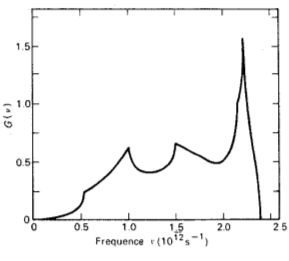
\includegraphics[scale=0.4]{ch7/image1.png}
	\captionof{figure}{ }
	\end{wrapfigure}
Si $g(\omega)$ est connu, on peut évaluer \autoref{eq:C(Tomega)} numériquement. 
Obtenir cette fonction n'est pas contre pas simple. Pour s'en convaincre, il 
suffit de regarder la fonction ci-contre. Il s'agit de la densité de mode 
reconstruite pour des cristaux de potassium.
soit le nombre de degrés de libertés.\\
A partir de cette expression, deux modèles vont apparaître :
\begin{itemize}
\item[$\bullet$] Le modèle d'Einstein qui suppose que tous les modes sont à
la même fréquence.
\item[$\bullet$] Le modèle de Debye qui suppose une relation de dispersion 
des phonons linéaires en $q$ dans la première zone de Brillouin.
\end{itemize}



	\subsection{Le modèle d'Einstein}
	Dans ce modèle, tous les atomes oscilles à la même fréquence $\omega_E$, 
	donnant lieu à une relation de dispersion indépendante de $q$\footnote{
	Alors représenté par une horizontale.}. Si le cristal possède $N$ mailles 
	et $r$ atomes par mailles, la densité d'état d'Einstein s'écrit
	\begin{equation}
	g_E(\omega) = 3rN\delta(\omega-\omega_E)
	\end{equation}
	Injectons cette relation dans \autoref{eq:C(Tomega)} et introduisons la 
	température d'Einstein 
	\begin{equation}
	k_B\theta_E = \hbar \omega_E
	\end{equation}
	de sorte à obtenir la chaleur spécifique d'Einstein
	\begin{equation}
	C_E(T) = 3rNk_B\left(\dfrac{\theta_E}{T}\right)^2\dfrac{e^{\theta_E/T}}{
	\left[\theta_E/T-1\right]^2}
	\end{equation}
	Pour des valeurs élevée, on obtient la valeur classique de Dulong et Petit
	(il faut développer le dénominateur  en série)
	\begin{equation}
	C_E(T) = 3rNk_B
	\end{equation}
	Ceci nous informe que nous avons $3rN$ modes et que chacun ont une 
	contribution de $k_B$ : \textbf{tous} les modes participent à haute énergie.

	\newpage
		\begin{wrapfigure}[10]{l}{5cm}
	\vspace{-0.2cm}
	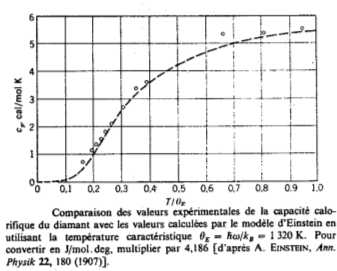
\includegraphics[scale=0.4]{ch7/image2.png}
	\captionof{figure}{ }
	\end{wrapfigure}
	Et pour basse température, l'exponentielle domine de sorte à avoir (formule 
	déduite à partir de Bose-Einstein) 
	\begin{equation}
	C_E(T) = 3rNk_B\left(\dfrac{\theta_E}{T}\right)^2e^{-\theta/T}
	\end{equation}
	Ceci est la première justification de la décroissance exponentielle de la 
	chaleur spécifique à basse température. Ceci est vrai  pour tous les solides. 
	Par contre, la valeur de $C(T)$ est sous-estimée à basse température à cause 
	de la non-considération des modes de vibrations acoustiques de très faibles 
	fréquences: ce modèle est bien meilleur pour les modes optiques.	



	\subsection{Le modèle de Debye}
	Son approximation est d'ignorer la dispersion (une seule vitesse de propagation 
	des ondes) et de remplacer les branches $\omega_{\vec{q}s}$ par 1! branche 
	acoustique
	\begin{equation}
	\omega = vq
	\end{equation}
	où $v$ est constante et la zone de Brillouin est remplacé par une  sphère. 
	Comme les valeurs permises de $q$ sont distribuées uniformément dans l'espace 
	réciproque :
	\begin{equation}
	g_D(q)\ dq \propto 4\pi q^2\ dq
	\end{equation}
	Et par conséquent
	\begin{equation}
	g_D(\omega) = B\omega^2
	\end{equation}
	Cette équations s'applique jusqu'à une fréquence maximale de sorte à toujours 
	vérifier (normalisation sur le nombre total de mode)
	\begin{equation}
	\int_0^{\omega_D} g_D(\omega)\ d\omega = 3rN
	\end{equation}
	On a alors
	\begin{equation}
	g_D(\omega) = 9rN\dfrac{\omega^2}{\omega_D^3}
	\end{equation}
	\begin{wrapfigure}[10]{r}{4.5cm}
	\vspace{-0.6cm}
	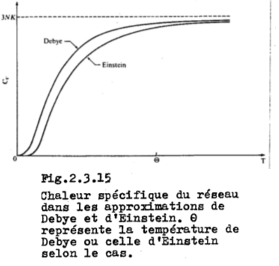
\includegraphics[scale=0.5]{ch7/image3.png}
	\captionof{figure}{ }
	\end{wrapfigure}
	ce qui est la distribution des fréquences dans l'approximation de Debye. En 
	introduisant la température de Debye et en posant
	\begin{equation}
	k_B\theta_B = \hbar\omega_D,\qquad x=\dfrac{\hbar\omega}{k_BT},\qquad x_D = 
	\dfrac{\hbar\omega_D}{k_BT}=\dfrac{\theta_D}{T}
	\end{equation}
	la chaleur spécifique devient
	\begin{equation}
	C_D(T) = 9rNk_B\left(\dfrac{T}{\theta_D}\right)^3\int_0^{x_D}\dfrac{x^4e^x}{
	\left[e^x-1\right]^2}\ dx
	\end{equation}
	Comme la valeur de l'intégrale dans $C_D(T)$ ne dépend que de $x_D=\theta_D/T$, 
	$C_D(T)$ doit être la même pour tous les matériaux.\\
	La chaleur spécifique d'Albert est bien plus faible que celle de Debye, reflétant 
	la difficulté d’exciter thermiquement des modes optiques à faible température.	
	A basse température, ce modèle est bien meilleur que celui d'Einstein. En effet, 
	$C_D(T)$ est bien plus grande que $C_E(T)$ à faible température.
	\begin{center}
	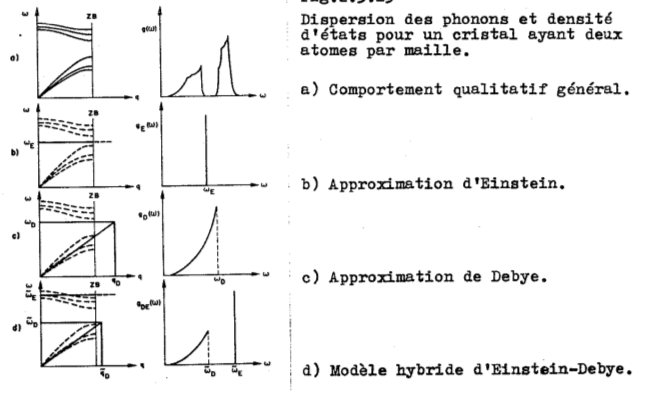
\includegraphics[scale=0.5]{ch7/image4.png}
	\captionof{figure}{ }
	\end{center}
	Reprenons les cas limites. Si $\theta_D \ll T$, on retrouve le résultat classique 
	(développement en série de $e^x,\dots$)
	\begin{equation}
	C_D(T) = 3rNk_B
	\end{equation}
	Si $T \rightarrow 0$, l'intégrale vaut $4\pi^4/15\approx 26$ et on trouve la loi 
	en $T^3$ de la chaleur spécifique d'un cristal à trois dimensions :
	\begin{equation}
	C_D(T) = \dfrac{12\pi^4}{5}rNk_B\left(\dfrac{T}{\theta_D}\right)^3,\qquad T \ll 
	\theta_D
	\end{equation}
	A basse température, ce sont donc principalement les phonons acoustiques qui vont 
	jouer (il faut une certaine température pour que les phonons optiques s'activent).\\
	Pour ces faibles températures, nous avons vu que Debye fonctionnait très bien, à 
	un tel point qu'il n'est pas pertinent de considérer Einstein ici. Par contre, ce 
	dernier sera plus pertinent pour l'étude des phonons optiques. On peut dès lors 
	constituer un modèle "hybride" : Debye pour l'acoustique, Einstein pour l'optique.
	

\section{L'effet Mössbauer}
Il s'agit d'un effet résultant de la combinaison entre un effet de la physique nucléaire 
et de la physique du solide. Supposons qu'un atome radioactif émette un phonon $\gamma$. 
Cette émission va faire "reculer" l'atome et le photon $\gamma$ émis n'aura pas 
exactement l'énergie de la transition.\\
Considérons un second atome qui "reçoit" le photon $\gamma$. Par le même effet que 
précédemment, cet atome va reculer dépensant un peu d'énergie. Pour avoir une transition 
électronique, il faut donc une énergie légèrement plus grande : il n'y a pas de 
recouvrement entre l'émission et la vibration.\\

Ceci est généralement vrai, sauf si on se trouve au sein d'un cristal : le mouvement de 
recul va se décomposer en un mouvement vibratoire, transmettant l'énergie de recul dans 
tout le cristal. Il existe une probabilité non nulle d'émission à zéro phonons : dans 
ce cas, la raie d’absorption vaut celle d'émission et aucune énergie n'est "perdue" 
en énergie cinétique.